\documentclass{article}

\usepackage{amsmath, amssymb, braket}
\usepackage{graphicx}
\graphicspath{{./images/}}

\newcommand{\Prob}[2]{P\left(#1\,|\,#2\right)}
\newcommand{\I}{\text{I}}
\newcommand{\X}{\text{X}}
\newcommand{\RX}{\mathrm{R_X}}
\newcommand{\Hgt}{\text{H}}
\newcommand{\Sgt}{\text{S}}
\newcommand{\CX}{\text{CX}}
\newcommand{\CCX}{\text{CCX}}

\author{Adrian Hall}
\title{Interaction-Free Measurement and Counterfactual Quantum Computation}

\begin{document}

\maketitle

In 1993, Elitzur and Vaidman put forward an interesting consequence of quantum mechanics that permits measurement of a physical system without interacting with it. The phenomenon can be nicely illustrated by a thought-experiment using a Mach-Zender interferometer, in which a single photon is used to detect the presence light-absorbing (or scattering) obstacle. In this report, I will explore the problem of interaction-free measurement and attempt to express it in the language of qubit operations as employed in the field of quantum computer science. In the process, I will demonstrate that this is a special case of counterfactual quantum computation, a counterintuitive phenomenon that permits ascertainment of the behavior of a quantum computer without actually running that computer.

\begin{figure} \label{fig:interferometer}
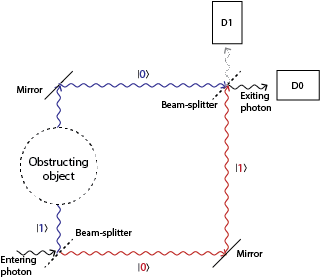
\includegraphics[scale=0.8]{mach-zender}
\centering
\caption{Mach-Zender interferometer, based on Elitzur and Vaidman (1993). Light enters in the rightward direction then passes through 45° beam-splitters and mirrors. An object may be positioned in the path of one beam.}
\end{figure}

A Mach-Zender interferometer (Fig. \ref{fig:interferometer}) is an optical device consisting of mirrors, beam splitters, and detectors, that is used to determine the relative phase difference between two paths taken by a stream of particle (generally, photons). Incoming light strikes the first beam-splitter, which partitions it into two paths; one travels upwards, the other rightwards. Both beams are reflected by mirrors, and finally incident on another beam-splitter. The intensities of the resultant two beams are measured by detectors $D0$ and $D1$. Each time the beam is reflected, it incurs a phase shift. It is possible to adjust the angles and positions of the mirrors slightly so that the path difference between the two beams is exactly one-half wavelength for the upward-traveling emitted light, resulting in destructive interference between the incoming waves, while the light exiting in the rightward direction exhibits constructive interference. This will cause an isolated interferometer to measure 100\% intensity at $D0$, and 0 intensity at $D1$.

In this specific case, we imagine a Mach-Zender interferometer optimized for handling a single photon. To describe this example in terms of qubit operations, we must assign qubit states to represent the photon's trajectory. Assuming the interferometer is working properly, the photon will always (classically) be going either up or to the right, which can be represented by a single bit. In reality, however, a photon can be in a superposition of taking both paths through the interferometer. To model this, we encode its direction as a single qubit can be in a superposition of two classical bit values, making it an apt choice to model this system. Let state $\ket 0$ represent a photon traveling in the rightward direction, and state $\ket 1$ represent a photon traveling upward.

The optical components present include 45° mirrors and beam-splitters, as well as a pair of photon detectors. To properly capture the system's behavior, we need to represent the effects of these devices as operations on a qubit. Simplest is the pair of fully-silvered mirrors, which converts each rightward-traveling photon to an upward-traveling one, and vice-versa. For a photon in superposition, it swaps the amplitudes of upward- and rightward-traveling components, sending $\ket 0 \to \ket 1$ and $\ket 1 \to \ket 0$, which means that the mirrors have the effect of applying the Pauli $\X$ gate to the traveling photon. As a side note, a physical consequence of the reflection of light by a mirror is that each reflected photon gains a phase of $\pi/2$. However, this global phase of $i$ is not observable, so we will ignore it.

The effect of each beam-splitter is to reflect half of the incident light and transmit the rest. To a single photon traveling purely in one direction, they have the effect of creating a superposition of upward and rightward travel. Here, the phase shift due to reflection is relative, since transmitted light is not shifted, so we must keep track of it:
$$\ket 0 \to \frac{\ket 0 + i\ket 1}{\sqrt{2}} \qquad \ket 1 \to \frac{i\ket 0 + \ket 1}{\sqrt{2}}$$
This operation can be written as:
$$2^{-1/2}\begin{pmatrix}1 && i \\ i && 1\end{pmatrix} = \cos\frac{\pi}{4}\I + i\sin\frac{\pi}{4}\X = \RX\left(-\frac{\pi}{2}\right)$$
Therefore, the Mach-Zender interferometer, in the absence of an obstructing object, performs the unitary transformation
$$U_0 = \RX\left(-\frac{\pi}{2}\right)\X\RX\left(-\frac{\pi}{2}\right)$$
The effect of the detectors is then to measure the state of the photon qubit after the interferometer has acted on it. A photon that leaves the second beam-splitter traveling right will strike $D0$, and one traveling up will strike $D1$.

Let's examine what happens when a photon traveling right enters the interferometer:
\begin{equation} \label{eq:seq_0}
\ket 0 \xrightarrow{\RX\left(-\frac{\pi}{2}\right)} \frac{\ket 0 + i\ket 1}{\sqrt{2}} \xrightarrow{\X} \frac{\ket 1 + i\ket 0}{\sqrt{2}} \xrightarrow{\RX\left(-\frac{\pi}{2}\right)} \frac{i\ket 0 + \ket 1 + i\ket 0 - \ket 1}{2} = i\ket 0
\end{equation}
And traveling up:
\begin{equation} \label{eq:seq_1}
\ket 1 \xrightarrow{\RX\left(-\frac{\pi}{2}\right)} \frac{i\ket 0 + \ket 1}{\sqrt{2}} \xrightarrow{\X} \frac{i\ket 1 + \ket 0}{\sqrt{2}} \xrightarrow{\RX\left(-\frac{\pi}{2}\right)} \frac{-\ket 0 + i\ket 1 + \ket 0 + i\ket 1}{2} = i\ket 1
\end{equation}
So, by linearity, the empty interferometer is equivalent to the transformation $i\I$; the direction of the exiting photon is unaltered. If a photon enters traveling to the right (in state $\ket 0$), it will strike detector $D0$ with 100\% probability. An optical description of this effect is to say that destructive interference between the two beams incident on the second beam-splitter cancels out the final upward-traveling component. As I will explain shortly, if one of these beams is obstructed, then this interference effect will not occur, permitting light to enter both detectors.

In order to represent the effect of an obstructing object, we need to keep track of additional information. Unlike the unobstructed system, absorption or scattering of a photon is not a reversible process, and therefore cannot be represented by a unitary transformation. Upon interaction, the obstructing object has the effect of coupling the photon's state to a noisy thermal environment, which in practice will cause a ``collapse'' to a classical state of having either interacted or not interacted. In the language of quantum computing, the interaction amounts to classical measurement of a quantum state.

We can use a second qubit to track whether or not an interaction has occurred. Let $q_0$ encode the photon probe's direction as described above, and let $q_1$ be in state $\ket 1$ if the photon is incident on the object, and state $\ket 0$ if no interaction occurs. In the presence of an object, an interaction will occur iff the photon is traveling up, so $q_1$ will change from $\ket 0 \to \ket 1$ iff $q_0 = \ket 1$. This can be modeled as a $\CX_{01}$ gate, meaning that the obstructed interferometer is equivalent to the transformation:
$$U_1 = \RX\left(-\frac{\pi}{2}\right)_0 \X_0 \, \CX_{01} \, \RX\left(-\frac{\pi}{2}\right)_0$$
Following the action of the above transformation, we will measure $q_1$ to induce a partial collapse. As above, let's examine the behavior for initial state $\ket{00}$, which represents the photon traveling right with no interaction having occurred yet.
\begin{multline} \label{eq:seq_00}
\ket{00} \xrightarrow{\RX\left(-\frac{\pi}{2}\right)_0} \frac{\ket{00} + i\ket{01}}{\sqrt{2}} \xrightarrow{\CX_{01}} \frac{\ket{00} + i\ket{11}}{\sqrt{2}}\\
\xrightarrow{\X_0} \frac{\ket{01} + i\ket{10}}{\sqrt{2}} \xrightarrow{\RX\left(-\frac{\pi}{2}\right)_0} \frac{i\ket{00} + \ket{01} + i\ket{10} - \ket{11}}{2}\\
= \frac{i}{\sqrt{2}}(\ket0 \otimes \ket{-i} + \ket1 \otimes \ket{+i})
\end{multline}

%\begin{multline*}
%\ket{01} \xrightarrow{R_X\left(-\frac{\pi}{2}\right)_0} \frac{i\ket{00} + \ket{01}}{\sqrt{2}} \xrightarrow{X_0} \frac{i\ket{01} + \ket{00}}{\sqrt{2}}\\
%\xrightarrow{CX_{01}} \frac{i\ket{11} + \ket{00}}{\sqrt{2}} \xrightarrow{R_X\left(-\frac{\pi}{2}\right)_0} \frac{-\ket{10} + i\ket{11} + \ket{00} + i\ket{01}}{2}\\
%= \frac{i}{\sqrt{2}}(\ket0 \otimes \ket{+i} - \ket1 \otimes \ket{-i})
%\end{multline*}
By comparing this sequence to Eq. \ref{eq:seq_0}, we can see that the where we had cancellation of $\ket 1$ and $-\ket 1$, we now have the linearly independent $\ket{01}$ and $-\ket{11}$. Measurement of $q_1$ in the computational basis gives:
$$q_1 \to 0: q_0 = \ket{-i} \qquad q_1 \to 1: q_0 = \ket{+i}$$
Unlike the unobstructed case, in which the photon always ends up traveling in the same direction that it started in, the obstructed interferometer has a 50\% chance of changing its direction of travel. Thus, it is possible for a photon fired in the rightward direction $\ket 0$ to trigger detector $D1$ iff there is an obstruction. It is particularly interesting that this is true whether or not the interaction occurs: even if $q_1$ measures to 0, $q_0$ will remain in a superposition of $\ket 0$ and $\ket 1$.

In summary, when an object is absent there is a 100\% chance that $D0$ triggers, and when an object is present, there is a 50\% chance of interaction (in which case no detector triggers), a 25\% chance that $D1$ triggers, and a 25\% chance that $D0$ triggers. In comparison, an ordinary measurement would have a 100\% chance of interaction, and a 100\% theoretical accuracy. If we do an interaction-free measurement like this, we can't be sure that we won't get a false negative result. If $D1$ triggers, or if we fire a photon and no detector triggers, then we know there is an object blocking the upward beam, but if $D0$ triggers, we cannot be sure. If the prior probability of an object being present is $p_1$, then Bayes' theorem tells us that in the event of $D0$ triggering, the probability that an object is present is:
$$\Prob{\text{object}}{D0} = \frac{p_1}{4 - 3 p_1} \qquad \Prob{\text{object}}{n \times D0} = \frac{p_1}{4^n - (4^n - 1) p_1}$$
And therefore if we want an upper bound of $1/\xi$ on the false negative rate, we need:
$$n = \frac{1}{2} \log_2 \left[ (\xi - 1) \frac{p_1}{1 - p_1}\right]$$
This means that for a given certainty threshold, our detection ``algorithm'' requires additional oracle calls proportional to the logarithm of the odds that an object is present.

It is possible to modify this process such that the false negative rate is zero. By applying the unitary operation $\Hgt\Sgt^\dagger$ to the final result pre-measurement, mapping:
$$\ket 0 \to \ket + \quad \ket 1 \to - i \ket - \qquad \ket{+i} \to \ket 0 \quad \ket{-i} \to \ket 1$$
If an interaction occurs, no photon emerges from the interferometer and we know for certain that an object is present. Referring to Eq. \ref{eq:seq_00}, if no interaction occurs but an object is present, the photon will exit the interferometer in state $\ket{-i}$. Applying $\Hgt\Sgt^\dagger$ transforms this to $\ket 1$, resulting in a 100\% probability that $D0$ will trigger. However, if no object is present, the photon exits in state $\ket 0$, which $\Hgt\Sgt$ transforms to $\ket +$, introducing a 50\% chance of $D1$ triggering (a false positive). This trade-off is inescapable: since $\ket 0$ and $\ket{-i}$ have a non-zero inner product, no unitary operation exists that maps them onto orthogonal states (which is required for perfectly accurate measurement).

\begin{figure}
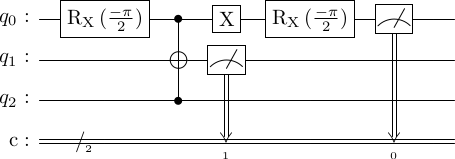
\includegraphics[scale=0.5]{circuit-render}
\centering
\caption{Quantum circuit rendering of the interferometer. Qubits 0-2 represent, respectively, the direction of the photon, the status of the interaction, and whether or not the object is obstructing the beam.}
\label{fig:circuit-render}
\end{figure}

We can combine the obstructed an unobstructed gates into a single quantum circuit (Fig. \ref{fig:circuit-render}) by adding a third qubit:
\begin{equation} \label{eq:unitary}
U = \ket 0\bra 0 \otimes U_0 + \ket 1\bra 1 \otimes U_1 = \RX\left(-\frac{\pi}{2}\right)_0 \X_0 \, \CCX_{021} \, \RX\left(-\frac{\pi}{2}\right)_0
\end{equation}
Where $\CCX_{021}$ is the Toffoli gate with controls on $q_0$ (photon direction) and $q_2$ (object presence) and target on $q_1$ (interaction occurrence). An interesting consequence of this formulation is that it allows us to examine the behavior of the system when the object is in a superposition of obstructing vs. not obstructing the beam. We can represent this as:
$$q_2 = \alpha \ket 0 + \beta \ket 1$$
Applying Eq. \ref{eq:unitary} gives:
\begin{equation}
\ket{q_2 0 0} \xrightarrow{U} \alpha\ket 0 \otimes i\ket{00} + \beta \ket 1 \otimes \frac{i}{\sqrt{2}}(\ket0 \otimes \ket{-i} + \ket1 \otimes \ket{+i})
\end{equation}
Since both $U_0$ and $U_1$ impart an individually unobservable global phase of $i$ , there is no phase kickback induced by the control. It is also worth noting that measurements of $(q_1, q_0)$ that give $(0, 1)$, $(1, 0)$ or $(1, 1)$ all correspond to eigenstates with $q_2 = \ket 1$, meaning that even in the absence of interaction, a positive measurement still induces collapse of $q_2$ to $\ket 1$. Overall, the measurement probabilities amount to:
$$\begin{array}{ r l l }
\text{eigenstate }\ket{1 1 q_0}: & P(\text{interaction}) & = \frac{\beta^2}{2} \\
\text{eigenstate }\ket{q_2 0 0}: & P(D0) & = 1 - \frac{3 \beta^2}{4} \\
\text{eigenstate }\ket{1 0 1}: & P(D1) & = \frac{\beta^2}{4}
\end{array}$$
The ratio $P(D1) : P(\text{interaction}) = 1 : 2$ is independent of $q_2$. Since $D1$ triggering represents an interaction-free measurement, this means the "counterfactual efficiency" of $U$ is limited: for every interaction-free measurement there will be, on average, two interactions.

These statistics can be improved by altering the properties of the beam-splitters. Previously, we used two identical splitters, each of which reflects and transmits equal intensities of light. We could in principle instead use two different beam splitters that perform the operations:
$$\RX(\theta) = \begin{pmatrix}
\cos(\theta / 2) && -i\sin(\theta / 2)\\
-i\sin(\theta / 2) && \cos(\theta / 2)
\end{pmatrix}$$
$$\mathrm{R^\prime_X(\theta)} = \begin{pmatrix}
\sin(\theta / 2) && -i\cos(\theta / 2)\\
-i\cos(\theta / 2) && \sin(\theta / 2)
\end{pmatrix}$$
\begin{figure} \label{fig:circuit-improved}
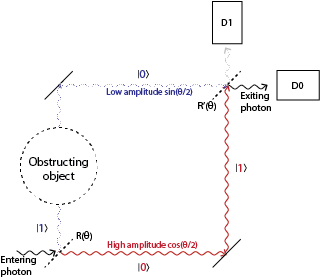
\includegraphics[scale=0.8]{mach-zender-improved}
\centering
\caption{Mach-Zender interferometer with altered beam splitters designed to divert most light away from the object for small values of $\theta$.}
\end{figure}
For a small $\theta$, $R_X$ mainly transmits, and $R^\prime_X$ mainly reflects. We can modify our unitary to use $R_X$ as the first splitter and $R^\prime_X$ as the second, the effect of which is to divert the majority of photon's amplitude away from the obstructing object (Fig. \ref{fig:circuit-improved}). The resulting transformation is:
$$U(\theta) = \mathrm{R^\prime_X(\theta)_0} \X_0 \CCX_{021} \RX(\theta)$$
Similarly to the original unitary $U(-\pi/2)$, the result of $U(\theta)$ acting on $\ket{q_200}$ (discarding a global phase of $-i$) is:
\begin{multline}
\alpha\ket{000} \\+ \beta \ket 1 \otimes \frac{1}{2}(\ket0 \otimes (\cos^2(\theta/2)\ket 0 + i \cos(\theta/2)\sin(\theta/2)\ket 1)\\+ \ket 1 \otimes (\sin^2(\theta/2)\ket 0 - i\cos(\theta/2)\sin(\theta/2)\ket 1)
\end{multline}
Here the probability of interaction (measuring $q_1 \to 1$) and of interaction-free measurement (measuring $q_1 \to 0$ and $q_0 \to 1$) are respectively:
$$\begin{aligned}
P(\text{interaction}) = && \sin^4(\theta/2) + \cos^2(\theta/2)\sin^2(\theta/2)\\
P(D1) = && \cos^2(\theta/2)\sin^2(\theta/2)\end{aligned}$$
And so:
$$\frac{P(D1)}{P(\text{interaction})} = \frac{1}{1 + \tan^2(\theta/2)}$$
This approaches 1 for small $\theta$, giving a lower limit of 50\% for the average fraction of measurements that result in interaction with the object being measured.

More recent research has demonstrated even more efficient methods of performing counterfactual computations using the Quantum Zeno effect, in which the interaction qubit is repeatedly rotated into a state with much greater $\ket 0$ amplitude than $\ket 1$ amplitude and then measured. Since measurement of $q_1$ does not erase the state of $q_0$, it is possible to gradually rotate $q_0$ into an arbitrarily high probability of measuring to 1, while maintaining a negligible probability of interaction. However, this process requires apparatus significantly more complex than the basic Mach-Zender setup, and I will not describe it in detail here.

I will however illustrate a potential application of interaction-free measurement, which is to reduce the effect of radiation damage in imaging techniques such as microscopy.
\end{document}